% ---
%% USPSC-Cap3-Citacoes.tex
% --
% Este capítulo traz os exemplos de citações das "Diretrizes para apresentação de dissertações e teses da USP: documento eletrônico e impresso - Parte I (ABNT)" disponílvel em: http://biblioteca.puspsc.usp.br/pdfFiles_Caderno_Estudos_9_PT_1.pdf


% --- 
\chapter{Results and Discussion}
\label{ch:disc}
% --- 
\subsection{Activity along time}\label{constDisc}
Regular patterns of activity were observed along time
in the scales of seconds, minutes, hours, days and months.
Histograms in each of the time scales were computed as were circular average and dispersion values, and the results are given in Tables~\ref{tab:circ}-\ref{tab:min2}. For example, uniform activity is found with respect to seconds, minutes and days of the months. Weekend days exhibit about half the activity of regular weekdays, and there is a peak of activity between 11am and noon.


\begin{table}
\caption{The rescaled circular mean $\theta_\mu'$ and the circular dispersion $\delta(z)$, described in Section~\ref{sec:mtime}, for different timescales. This example table was constructed using all LAD messages, and the results are the same for other lists, as shown in Section~\ref*{si:circ} of the Supporting Information document. The most uniform distribution of activity was found in seconds and minutes. 	Hours of the day exhibited the most concentrated activity (lowest $\delta(z)$), with mean between 2 p.m. and 3 p.m. ($\theta'=-9.61$). Weekdays, days of the month and months have mean near zero (i.e. near the beginning of the week, month and year) and high dispersion. Note that $\theta_u'$ has the dimensional unit of the corresponding time period while $\delta(z)$ is dimensionless.}
\begin{center}
\begin{tabular}{ |l|| c|c| }
\hline
%scale & $\theta_\mu'$ & $S(z)$ & $Var(z)$ & $\delta(z)$ & $\frac{max(incidence)}{min(incidence)}$ & $ \mu_{\frac{max(incidence')}{min(incidence')}} $ & $ \sigma_{\frac{max(incidence')}{min(incidence')} } $ \\ \hline\hline
%& $\theta_\mu'$ & $S(z)$ & $Var(z)$ & $\delta(z)$  \\ \hline\hline
scale & mean $\theta_\mu'$ & dispersion $\delta(z)$  \\ \hline
seconds    & --//--  & 9070.17     \\\hline
minutes    & --//--  & 205489.40   \\\hline
hours      & -9.61   & 4.36        \\\hline
weekdays   & -0.03   & 29.28       \\\hline
month days & -2.65   & 2657.77     \\\hline
months     & -0.56   & 44.00       \\\hline

\end{tabular}
\end{center}
\label{tab:circ}
\end{table}

\begin{table}
\caption{Activity percentages along the hours of the day. Nearly identical distributions were observed on other social systems as shown in Section~\ref*{si:hours} of the Supporting Information document.
Highest activity was observed between noon and 6pm (with 1/3 of total day activity), followed by the time period between 6pm and midnight.
Around 2/3 of the activity takes place from noon to midnight
but the activity peak occurs between 11 a.m. and 12 p.m.
This table shows results for the activity in CPP.}
\footnotesize
\begin{center} 
 \begin{tabular}{ l || c | c | c | c | c | c }\hline
  & 1h & 2h & 3h & 4h & 6h & 12h \\\hline \hline
 0h  &  \multirow{1}{*}{ 3.66 }   &  \multirow{2}{*}{ 6.42 }   &  \multirow{3}{*}{ 8.20 }   &  \multirow{4}{*}{ 9.30 }   &  \multirow{6}{*}{ 10.67 }   &  \multirow{12}{*}{ 33.76 }  \\\cline{2-2} 
 1h  &  \multirow{1}{*}{ 2.76 }   &   &   &   &   &  \\\cline{2-2}\cline{3-3} 
 2h  &  \multirow{1}{*}{ 1.79 }   &  \multirow{2}{*}{ 2.88 }   &   &   &   &  \\\cline{2-2}\cline{4-4} 
 3h  &  \multirow{1}{*}{ 1.10 }   &   &  \multirow{3}{*}{ 2.47 }   &   &   &  \\\cline{2-2}\cline{3-3}\cline{5-5} 
 4h  &  \multirow{1}{*}{ 0.68 }   &  \multirow{2}{*}{ 1.37 }   &   &  \multirow{4}{*}{ 3.44 }   &   &  \\\cline{2-2} 
 5h  &  \multirow{1}{*}{ 0.69 }   &   &   &   &   &  \\\cline{2-2}\cline{3-3}\cline{4-4}\cline{6-6} 
 6h  &  \multirow{1}{*}{ 0.83 }   &  \multirow{2}{*}{ 2.07 }   &  \multirow{3}{*}{ 4.35 }   &   &  \multirow{6}{*}{ 23.09 }   &  \\\cline{2-2} 
 7h  &  \multirow{1}{*}{ 1.24 }   &   &   &   &   &  \\\cline{2-2}\cline{3-3}\cline{5-5} 
 8h  &  \multirow{1}{*}{ 2.28 }   &  \multirow{2}{*}{ 6.80 }   &   &  \multirow{4}{*}{ 21.03 }   &   &  \\\cline{2-2}\cline{4-4} 
 9h  &  \multirow{1}{*}{ 4.52 }   &   &  \multirow{3}{*}{ 18.75 }   &   &   &  \\\cline{2-2}\cline{3-3} 
 10h  &  \multirow{1}{*}{ 6.62 }   &  \multirow{2}{*}{ \textbf{ 14.23 } }   &   &   &   &  \\\cline{2-2} 
 11h  &  \multirow{1}{*}{ \textbf{ 7.61 } }   &   &   &   &   &  \\\cline{2-2}\cline{3-3}\cline{4-4}\cline{5-5}\cline{6-6}\cline{7-7} 
 12h  &  \multirow{1}{*}{ 6.44 }   &  \multirow{2}{*}{ 12.48 }   &  \multirow{3}{*}{ \textbf{ 18.95 } }   &  \multirow{4}{*}{ \textbf{ 25.05 } }   &  \multirow{6}{*}{ \textbf{ 37.63 } }   &  \multirow{12}{*}{ \textbf{ 66.24 } }  \\\cline{2-2} 
 13h  &  \multirow{1}{*}{ 6.04 }   &   &   &   &   &  \\\cline{2-2}\cline{3-3} 
 14h  &  \multirow{1}{*}{ 6.47 }   &  \multirow{2}{*}{ 12.57 }   &   &   &   &  \\\cline{2-2}\cline{4-4} 
 15h  &  \multirow{1}{*}{ 6.10 }   &   &  \multirow{3}{*}{ 18.68 }   &   &   &  \\\cline{2-2}\cline{3-3}\cline{5-5} 
 16h  &  \multirow{1}{*}{ 6.22 }   &  \multirow{2}{*}{ 12.58 }   &   &  \multirow{4}{*}{ 23.60 }   &   &  \\\cline{2-2} 
 17h  &  \multirow{1}{*}{ 6.36 }   &   &   &   &   &  \\\cline{2-2}\cline{3-3}\cline{4-4}\cline{6-6} 
 18h  &  \multirow{1}{*}{ 6.01 }   &  \multirow{2}{*}{ 11.02 }   &  \multirow{3}{*}{ 15.88 }   &   &  \multirow{6}{*}{ 28.61 }   &  \\\cline{2-2} 
 19h  &  \multirow{1}{*}{ 5.02 }   &   &   &   &   &  \\\cline{2-2}\cline{3-3}\cline{5-5} 
 20h  &  \multirow{1}{*}{ 4.85 }   &  \multirow{2}{*}{ 9.23 }   &   &  \multirow{4}{*}{ 17.59 }   &   &  \\\cline{2-2}\cline{4-4} 
 21h  &  \multirow{1}{*}{ 4.38 }   &   &  \multirow{3}{*}{ 12.73 }   &   &   &  \\\cline{2-2}\cline{3-3} 
 22h  &  \multirow{1}{*}{ 4.06 }   &  \multirow{2}{*}{ 8.36 }   &   &   &   &  \\\cline{2-2} 
 23h & \multirow{1}{*}{ 4.30 }  & & & & & \\\cline{2-2}\cline{3-3}\cline{4-4}\cline{5-5}\cline{6-6}\cline{7-7} 
 \hline\end{tabular} 
 \end{center}

\label{tab:hin}
\end{table}


\begin{table}
\caption{Activity percentages along weekdays.
Higher activity was observed during workweek days, with a decrease of activity on weekend days of at least one third and at most two thirds.}
\begin{center}
\begin{tabular}{ | l ||  c | c | c | c | c |   c | c |}
\hline
& Mon & Tue & Wed & Thu & Fri & Sat & Sun  \\ \hline
LAU & 15.71  & 15.81  & 15.88  & 16.43  & 15.14  & {\bf 10.13}  & {\bf 10.91} \\
LAD & 14.92  & 17.75  & 17.01  & 15.41  & 14.21  & {\bf 10.40}  & {\bf 10.31} \\
MET & 17.53  & 17.54  & 16.43  & 17.06  & 17.46  & {\bf 7.92 }  & {\bf 6.06 } \\
CPP & 17.06  & 17.43  & 17.61  & 17.13  & 16.30  & {\bf 6.81 }  & {\bf 7.67 } \\\hline

\end{tabular}
\end{center}
\label{tab:win}
\end{table}

In the scales of seconds and minutes, activity is uniform,
with the messages being slightly more evenly distributed in all lists than in simulations with the uniform distribution\footnote{Numpy version 1.8.2, ``random.randint'' function, was used for simulations, algorithms in \url{https://github.com/ttm/percolation}.}.
In the networks, $\frac{min(incidence)}{max(incidence)} \in (0.784,.794)$ while simulations reach these values but have on average more discrepant higher and lower peaks, i.e. if $\xi=\frac{min(incidence')}{max(incidence')}$ than $\mu_\xi=0.7741 \text{ and } \sigma_\xi=0.02619$.
Therefore, the incidence of messages at each second of a minute and at each minute of an hour was considered uniform.
In these cases, the circular dispersion is maximized and the mean has little meaning as indicated in Table~\ref{tab:circ}.
As for the hours of the day, an abrupt peak is found between 11am and 12pm with the most active period being the afternoon, with one third of total daily activity, and two thirds of activity are allocated in the second 12h of each day. Days of the week revealed a decrease between one third and two thirds of activity on weekends.
Days of the month were regarded as homogeneous with an inconclusive slight tendency of the first week to be more active.
Months of the year revealed patterns matching usual work and academic calendars. The time period examined here was not sufficient for the analysis of activity along the years. These patterns are exemplified in Tables~\ref{tab:hin}-\ref{tab:min2}.


\FloatBarrier

\begin{table}
\caption{Activity along the days of the month cycle.
Nearly identical distributions are found in all systems
as indicated in Section~\ref*{si:monthdays} of the Supporting Information. Although slightly higher activity rates are found in the beginning of the month, the most important feature seems to be the homogeneity made explicit by the high circular dispersion in Table~\ref{tab:circ}.
This specific example and empirical table correspond to the activity of the MET email list.}
\footnotesize
\begin{center}
\begin{tabular}{l || c | c | c | c}\hline
 & 1 day & 5 & 10 & 15 days \\\hline\hline
1 & \multirow{1}{*}{ 3.05 }  & \multirow{5}{*}{ 18.25 }  & \multirow{10}{*}{ 35.24 }  & \multirow{15}{*}{ 50.96 }  \\\cline{2-2}
2 & \multirow{1}{*}{ 3.38 }  & & & \\\cline{2-2}
3 & \multirow{1}{*}{ 3.62 }  & & & \\\cline{2-2}
4 & \multirow{1}{*}{ 4.25 }  & & & \\\cline{2-2}
5 & \multirow{1}{*}{ 3.94 }  & & & \\\cline{2-2}\cline{3-3}
6 & \multirow{1}{*}{ 3.73 }  & \multirow{5}{*}{ 16.98 }  & & \\\cline{2-2}
7 & \multirow{1}{*}{ 3.17 }  & & & \\\cline{2-2}
8 & \multirow{1}{*}{ 3.26 }  & & & \\\cline{2-2}
9 & \multirow{1}{*}{ 3.56 }  & & & \\\cline{2-2}
10 & \multirow{1}{*}{ 3.26 }  & & & \\\cline{2-2}\cline{3-3}\cline{4-4}
11 & \multirow{1}{*}{ 3.81 }  & \multirow{5}{*}{ 15.73 }  & \multirow{10}{*}{ 31.98 }  & \\\cline{2-2}
12 & \multirow{1}{*}{ 2.91 }  & & & \\\cline{2-2}
13 & \multirow{1}{*}{ 3.30 }  & & & \\\cline{2-2}
14 & \multirow{1}{*}{ 2.75 }  & & & \\\cline{2-2}
15 & \multirow{1}{*}{ 2.95 }  & & & \\\cline{2-2}\cline{3-3}\cline{5-5}
16 & \multirow{1}{*}{ 3.36 }  & \multirow{5}{*}{ 16.25 }  & & \multirow{15}{*}{ 49.04 }  \\\cline{2-2}
17 & \multirow{1}{*}{ 3.16 }  & & & \\\cline{2-2}
18 & \multirow{1}{*}{ 3.44 }  & & & \\\cline{2-2}
19 & \multirow{1}{*}{ 3.36 }  & & & \\\cline{2-2}
20 & \multirow{1}{*}{ 2.93 }  & & & \\\cline{2-2}\cline{3-3}\cline{4-4}
21 & \multirow{1}{*}{ 3.20 }  & \multirow{5}{*}{ 15.79 }  & \multirow{10}{*}{ 32.78 }  & \\\cline{2-2}
22 & \multirow{1}{*}{ 3.11 }  & & & \\\cline{2-2}
23 & \multirow{1}{*}{ 3.60 }  & & & \\\cline{2-2}
24 & \multirow{1}{*}{ 2.74 }  & & & \\\cline{2-2}
25 & \multirow{1}{*}{ 3.13 }  & & & \\\cline{2-2}\cline{3-3}
26 & \multirow{1}{*}{ 3.13 }  & \multirow{5}{*}{ 16.99 }  & & \\\cline{2-2}
27 & \multirow{1}{*}{ 3.07 }  & & & \\\cline{2-2}
28 & \multirow{1}{*}{ 3.61 }  & & & \\\cline{2-2}
29 & \multirow{1}{*}{ 3.60 }  & & & \\\cline{2-2}
30 & \multirow{1}{*}{ 3.57 }  & & & \\\cline{2-2}\cline{3-3}\cline{4-4}\cline{5-5}
\hline\end{tabular}
\end{center}

\label{tab:min}
\end{table}

\begin{table}
\caption{Activity percentages on months along the year. 	Activity is usually concentrated in Jun-Aug and/or in Dec-Mar, potentially due to academic calendars, vacations and end-of-year holidays. This table corresponds to activity in LAU. Similar results are shown for other lists in Section~\ref*{si:months} of the Supporting Information document.}
\footnotesize
\begin{center}
\begin{tabular}{| l || c | c | c | c | c |}\hline
 & m. & b. & t. & q. & s. \\\hline
Jan & \multirow{1}{*}{ 10.22 }  & \multirow{2}{*}{ 19.56 }  & \multirow{3}{*}{ 28.24 }  & \multirow{4}{*}{ 35.09 }  & \multirow{6}{*}{ 49.16 }  \\\cline{2-2}
Fev & \multirow{1}{*}{ 9.34 }  & & & & \\\cline{2-2}\cline{3-3}
Mar & \multirow{1}{*}{ 8.67 }  & \multirow{2}{*}{ 15.53 }  & & & \\\cline{2-2}\cline{4-4}
Apr & \multirow{1}{*}{ 6.86 }  & & \multirow{3}{*}{ 20.93 }  & & \\\cline{2-2}\cline{3-3}\cline{5-5}
Mai & \multirow{1}{*}{ 7.28 }  & \multirow{2}{*}{ 14.07 }  & & \multirow{4}{*}{ 30.36 }  & \\\cline{2-2}
Jun & \multirow{1}{*}{ 6.80 }  & & & & \\\cline{2-2}\cline{3-3}\cline{4-4}\cline{6-6}
Jul & \multirow{1}{*}{ 8.97 }  & \multirow{2}{*}{ 16.29 }  & \multirow{3}{*}{ 24.47 }  & & \multirow{6}{*}{ 50.84 }  \\\cline{2-2}
Ago & \multirow{1}{*}{ 7.32 }  & & & & \\\cline{2-2}\cline{3-3}\cline{5-5}
Set & \multirow{1}{*}{ 8.18 }  & \multirow{2}{*}{ 16.25 }  & & \multirow{4}{*}{ 34.55 }  & \\\cline{2-2}\cline{4-4}
Out & \multirow{1}{*}{ 8.06 }  & & \multirow{3}{*}{ 26.36 }  & & \\\cline{2-2}\cline{3-3}
Nov & \multirow{1}{*}{ 7.64 }  & \multirow{2}{*}{ 18.30 }  & & & \\\cline{2-2}
Dez & \multirow{1}{*}{ 10.66 }  & & & & \\\cline{2-2}\cline{3-3}\cline{4-4}\cline{5-5}\cline{6-6}
\hline\end{tabular}
\end{center}
\label{tab:min2}
\end{table}


\subsection{Stable sizes of Erd\"os sectors}\label{subsec:pih}

The distribution of vertices in the hub, intermediary, periphery Erd\"os sectors is remarkably stable along time if the snapshots hold 200 or more messages, as it is clear in Figure~\ref{fig:sectIL} and in Section~\ref*{si:frac} of the Supporting Information document. 
%Moreover, all email lists analyzed exhibit the same distribution profile.
Activity is highly concentrated on the hubs, while a very large number of peripheral vertices contribute to only a fraction of the activity.
This is expected for a system with a scale-free profile, as confirmed with the distribution of activity among participants in Table~\ref{autores}.

Typically, $[3\%-12\%]$ of the vertices are hubs,\\
$[15\%-45\%]$ are intermediary and $[44\%-81\%]$ are peripheral,
which is consistent with other studies~\cite{secFree}.
These results hold for the total, in and out degrees and strengths.
Stable sizes are also observed for 100 or less messages if the classification 
of the three sectors is performed with one of the compound criteria established in Section~\ref{sectioning}. The networks often hold this basic structure with as few as 10-50 messages, i.e. concentration of activity and the abundance of low-activity participants take place even with very few messages, which is highlighted in Section~\ref*{si:frac} of the Supporting Information. A minimum window size for the observation of more general properties might be inferred by monitoring 
both the giant component and the degeneration of the Erd\"os sectors.

In order to support the generality of these findings,
we list the Erd\"os sector sizes of 12 networks from Facebook, Twitter and Participabr in Table~\ref*{tab:secE} of the Supporting Information document. The fractions of hubs, intermediary and periphery nodes are
essentially the same as for the email list networks but with exceptions and a greater variability.

\begin{figure*} 
\centering
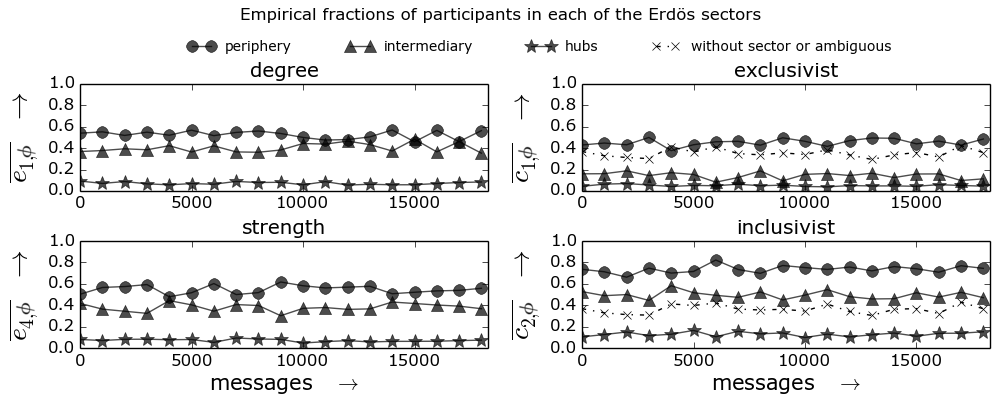
\includegraphics[width=\textwidth]{figs/InText-WLAU-S1000__}
\caption{Stability of Erd\"os sector sizes.
Fractions of participants derived from degree and strength criteria, $E_1$ and $E_4$ described in Section~\ref{sectioning}, are both on the left.
Fractions derived from the exclusivist $C_1$ and the inclusivist $C_2$ compound criteria are shown in the plots to the right.
The ordinates $\overline{e_{\gamma,\phi}}=\frac{|e_{\gamma,\phi}|}{N}$ denote the fraction of participants in sector $\phi$ through criterion $E_\gamma$
and, similarly, $\overline{c_{\delta,\phi}}=\frac{|c_{\delta,\phi}|}{N}$ denotes the fraction of participants in sector $\phi$ through criterion $C_\delta$.
Sections~\ref*{si:frac} and~\ref*{si:ext} of the Supporting Information bring a systematic collection of such timeline figures with all simple and compound criteria specified in Section~\ref{sectioning}, with results for networks from Facebook, Twitter and Participabr.}
\label{fig:sectIL}
\end{figure*}


\begin{table}[h]
\caption{Distribution of activity among participants.
The first column shows the percentage of messages sent by the most active participant. The column for the first quartile ($Q_1$) gives the minimum percentage of participants responsible for at least 25\% of total messages with the actual percentage in parentheses. Similarly, the column for the first three quartiles $Q_3$ gives the minimum percentage of participants responsible for 75\% of total messages.
The last decile $D_{-1}$ column shows the maximum percentage of participants responsible for 10\% of messages.}
\begin{center}
\begin{tabular}{ | l ||  c | c | c | c | }
\hline
list & hub & $ Q_1 $ & $ Q_3 $ & $D_{-1}$ \\ \hline
LAU & 2.78  & 1.19 (26.35\%)  & 13.12 (75.17\%)  & 67.32 (-10.02\%) \\
LAD & 4.00  & 1.03 (26.64\%)  & 11.91 (75.18\%)  & 71.14 (-10.03\%) \\
MET & 11.14  & 1.02 (34.07\%)  & 8.54 (75.64\%)  & 80.49 (-10.02\%) \\
CPP & 14.41  & 0.29 (33.24\%)  & 4.18 (75.46\%)  & 83.65 (-10.04\%) \\\hline

\end{tabular}
\end{center}
\label{autores}
\end{table}


\subsection{Stability of principal components}\label{prevalence}
%The topology was analyzed using standard, well-established metrics of centrality and clustering.
%We also introduced symmetry metrics given the evidence of their importance in social contexts~\cite{newmanEvolving}.
%The contribution of each metric to the variance is very similar for all the networks and along time.

The principal components of the participants are very stable in the topological space, i.e. in the space of principal components of network measures.
Table~\ref{tab:pcain} exemplifies the formation of principal components by providing the averages over non-overlapped activity snapshots of a network. The most important result of this application of PCA, the stability of principal components, is underpinned by the very small dispersion of the contribution of each metric to each principal component.
%The contribution of each metric to the
%principal components presents
%very small standard deviation.

\begin{table}[!h]
\caption{Loadings for the 14 metrics into the principal components for the MET list, $1000$ messages in 20 disjoint positions. The clustering coefficient (cc) appears as the first metric in the table, followed by 7 centrality metrics and 6 symmetry-related metrics. Note that the centrality measurements, including degrees, strength and betweenness centrality, are the most important contributors for the first principal component, while the second component is dominated by symmetry metrics. The clustering coefficient is only relevant for the third principal component. The three components have in average more than 85\% of the variance.
The low standard deviation $\sigma$ implies that the principal components are considerably stable.}
\footnotesize
\begin{center}
\begin{tabular}{| l || c | c | c | c | c | c |}\cline{2-7}
\multicolumn{1}{c|}{} & \multicolumn{2}{c|}{PC1}          & \multicolumn{2}{c|}{PC2} & \multicolumn{2}{c|}{PC3}  \\\cline{2-7}\multicolumn{1}{c|}{} & $\mu$            & $\sigma$ & $\mu$         & $\sigma$ & $\mu$ & $\sigma$  \\\hline
$cc$ &                     0.89  & 0.59  & 1.93  & 1.33  & {\bf 21.22}  & 2.97 \\\hline
$s$ &              {\bf 11.71}  & 0.57  & 2.97  & 0.82  & 2.45  & 0.72 \\
$s^{in}$ &         {\bf 11.68}  & 0.58  & 2.37  & 0.91  & 3.08  & 0.78 \\
$s^{out}$ &        {\bf 11.49}  & 0.61  & 3.63  & 0.79  & 1.61  & 0.88 \\
$k$ &              {\bf 11.93}  & 0.54  & 2.58  & 0.70  & 0.52  & 0.44 \\
$k^{in}$ &         {\bf 11.93}  & 0.52  & 1.19  & 0.88  & 1.41  & 0.71 \\
$k^{out}$ &        {\bf 11.57}  & 0.61  & 4.34  & 0.70  & 0.98  & 0.66 \\
$bt$ &             {\bf 11.37}  & 0.55  & 2.44  & 0.84  & 1.37  & 0.77 \\\hline
$asy$ &                    3.14  & 0.98  & {\bf 18.52}  & 1.97  & 2.46  & 1.69 \\
$\mu^{asy}$              & 3.32  & 0.99  & {\bf 18.23}  & 2.01  & 2.80  & 1.82 \\
$\sigma^{asy}$           & 4.91  & 0.59  & 2.44  & 1.47  & {\bf 26.84}  & 3.06 \\
$dis$                    & 2.94  & 0.88  & {\bf 18.50}  & 1.92  & 3.06  & 1.98 \\
$\mu^{dis}$              & 2.55  & 0.89  & {\bf 18.12}  & 1.85  & 1.57  & 1.32 \\
	$\sigma^{dis}$           & 0.57  & 0.33  & 2.74  & 1.63  & {\bf 30.61}  & 2.66 \\\hline\hline
$\lambda$                & 49.56 & 1.16  & 27.14  & 0.54  & 13.25  & 0.95 \\
\hline\end{tabular}
\end{center}

\label{tab:pcain}
\end{table}

The first principal component is an average of centrality metrics:
degrees, strengths and betweenness centrality.
On one hand, the similar relevance of all centrality metrics is not surprising since they are highly correlated,
e.g. degree and strength have Spearman correlation coefficient $\in [0.95,1]$ 
and Pearson coefficient $\in [0.85,1)$ for window sizes greater than a thousand messages.
On the other hand, each of these metrics is related to a different participation characteristic,
and their equal relevance for variability,
as measured by the principal component, is noticeable.
Also, this suggests that these centrality metrics 
are equally adequate for characterizing the networks
and the participants.

\begin{figure} 
\centering
%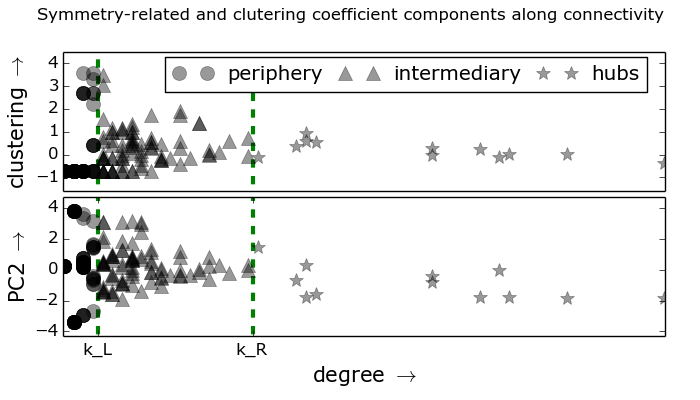
\includegraphics[width=.6\textwidth,height=10cm]{figs/im13PCAPLOT__}
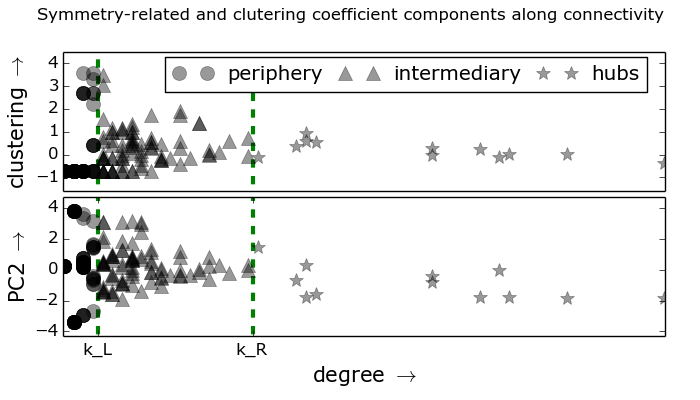
\includegraphics[width=.45\textwidth]{figs/im13PCAPLOT__}
\caption{The first plot highlights the well-known pattern of degree versus clustering coefficient, characterized by the higher clustering coefficient of lower degree vertices.
    The second plot shows the greater dispersion of the symmetry-related ordinates dominant in the second principal component (PC2).
This larger dispersion suggests that symmetry-related metrics are more powerful,
for characterizing interaction networks than the clustering coefficient,
especially for hubs and intermediary vertices.
This figure reflects a snapshot of the LAU list with 1000 contiguous messages.}

%		Similar structures were observed in all window sizes $ws\;\in\;[500,10000]$, in networks derived from email lists,
%		and in networks from Facebook, Twitter and Participabr,
%		which suggests a common relationship between the metrics of degrees, strengths and betweenness centrality,
%		the symmetry-related metrics and clustering coefficient.}
\label{fig:sym}
\end{figure}

According to Table~\ref{tab:pcain} and Figure~\ref{fig:sym},
dispersion is larger in symmetry-related metrics than in clustering coefficient.
% As expected from basic complex network theory, peripheral vertices have low values of centrality metrics and larger dispersion with regard to the clustering coefficient.
% %The scatter plot in the third system of Figure~\ref{fig:sym},
% %where all metrics are considered and there is a greater dispersion
% %with respect to the ordinates,
% This reflects in the relevance of the symmetry-related metrics.
We conclude that the symmetry metrics are more powerful, in terms of dispersion in the topological metrics space, in characterizing interaction networks and their participants, than the clustering coefficient, especially for hubs and intermediary vertices (peripheral vertices have larger dispersion with regard to the clustering coefficient).
Interestingly, the clustering coefficient is always combined
with the standard deviation of the asymmetry and disequilibrium
of edges $\sigma^{asy}$ and $\sigma^{dis}$ in the third principal component.

%These results are also reported for 12 networks from Facebook, Twitter and Participabr
%in Section~\ref{si:ext} of the Supporting Information document.
Similar results are presented in Sections~\ref*{si:pcat} and~\ref*{si:ext}
of the Supporting Information for other email lists and interaction networks. A larger variability was found for the latter networks,
which motivated the use of interaction networks derived from email lists for benchmarking.

%the overall behavior was maintained in that centrality measurements 
%were found prevalent in the first principal component,
%followed by symmetry-related metrics on the second principal
%component and then clustering coefficient on the third principal component.
%Similar results are presented in Sections~\ref{si:pcat} and~\ref{si:ext}
%of the Supporting Information document for other email lists and other interaction networks,
%with the consideration of strategic combinations of metrics.

\subsection{Types from Erd\"os sectors}\label{sec:pty}


Assigning a type to a participant raises important issues about the scientific cannon for human types and the potential for stigmatization and prejudice. The Erd\"os sector to which a participant belongs can be regarded as implying a social type for this participant.
In this case, the type of a participant changes both along time and as different networks are considered, despite the stability of the network. Therefore, the potential for prejudice of such participant typology is attenuated~\cite{adorno}. In other words, an individual is a hub in a number of networks and peripheral in other networks, and even within the same network he/she most probably changes type along time~\cite{animacoes}.

The importance of this issue can be grasped by the consideration of static types derived from quantitative criteria. For example, in email lists with a small number of participants, the number of threads has a negative correlation with the number of participants.
When the number of participants exceeds a threshold, the number of threads has a positive correlation with the number of participants.
This finding is illustrated in Figure~\ref{fig:nmgamma3d}
and can also be observed in Table~\ref{tab:genLists}.
The assignment of types to individuals, in this latter case,
has more potential for prejudice because
the derived participant type is static and
one fails to acknowledge that
human individuals are not immutable entities.

Further observations regarding the Erd\"os sectors
and the implicit participant types were made, which are consistent with the literature~\cite{barabasiEvo}: 1) hubs and intermediary participants usually have intermittent activity, and stable activity was found only in smaller communities. For instance, the MET list had stable hubs while LAU, LAD and CPP exhibited intermittent hubs.
2) Network structure seems to be most influenced by the
activity of intermediary participants as they have less extreme
roles than hubs and peripheral participants and
can therefore connect to the sectors and other participants 
in a more selective and explicit manner.




%Moreover, such typology of participants bridges exact and human sciences and may 
%be enriched with concepts from other typologies,
%such as Meyer-Briggs, Pavlov or the authoritarian types of the F-Scale~\cite{adorno}.

%We analyzed the temporal evolution of the networks
%using visualization
%tools developed for this research~\cite{rcText,versinus}
%and inspected raw data.

%dictated (or revealed) by the
%(e.g. stable or intermittent patterns of activity and preferential communication
%with hubs or periphery)

%of both hubs and peripheral vertices
%have the trivial facets of interacting 
%
%
%
%\begin{itemize}
%	\item Typically, the activity of hubs is trivial: they interact as much as possible, in every occasion with everyone.
%The activity of peripheral vertices also follows a simple pattern: they interact very rarely, in very few occasions.
%Therefore, intermediary vertices seem responsible for the network structure.
%Intermediary vertices may exhibit preferential communication to peripheral, intermediary, or hub vertices; can be marked by stable communication partners; can involve stable or intermittent patterns of activity, to point just a few examples of this greater variety of roles.
%%	\item Some of the most active participants receive many responses with relative few messages sent, and rarely are top hubs.
%%These seem as authorities and contrast with participants that respond much more than receive responses.
%%	\item The most obvious community structure, as observed by a high clustering coefficient, i.e. members know each other often, is found mostly in peripheral and intermediary sectors.
%\end{itemize}

%Within networks as the whole objects of analysis,
%we were able to observe a peculiar correlation pattern 
%between the number of threads and the number of participants.
\begin{figure}
\centering
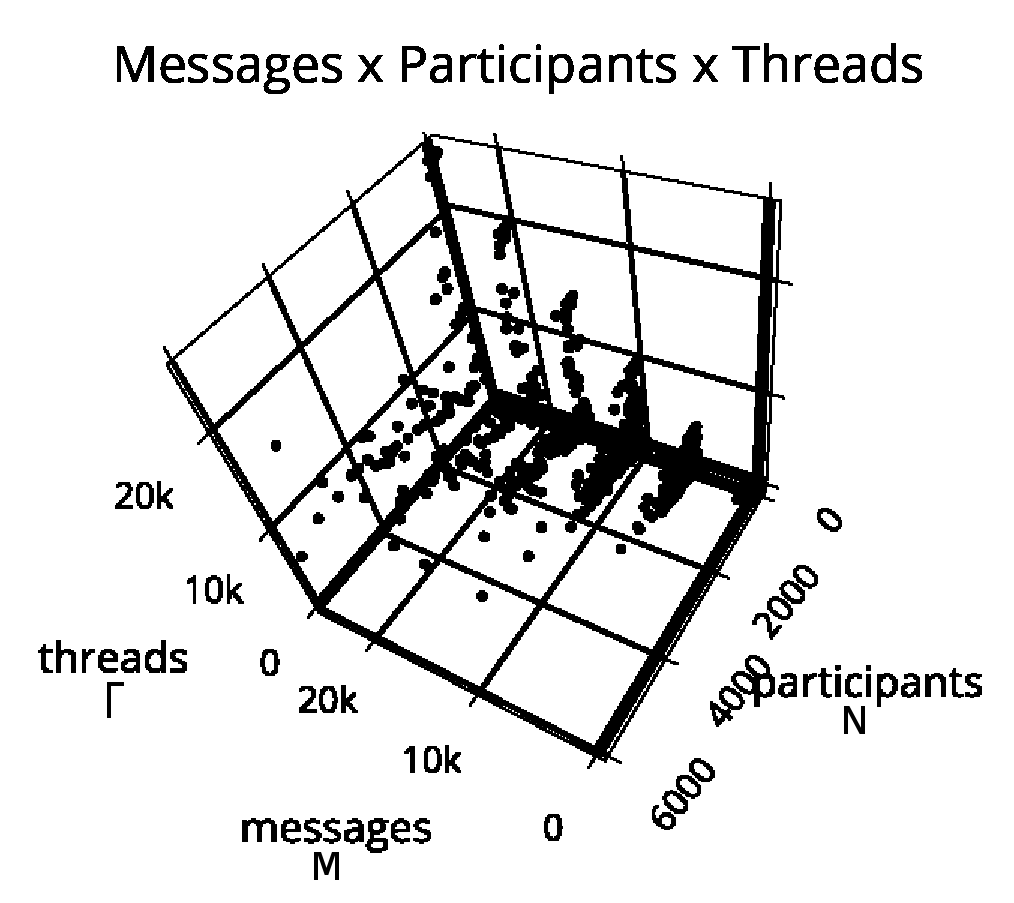
\includegraphics[trim={0 0 0 1cm},clip,width=.7\columnwidth]{figs/mpgamma2_}
\caption{A scatter plot of number of messages $M$ versus number of participants $N$ versus number of threads $\Gamma$ for 140 email lists.
Highest $\Gamma$ is associated with low $N$.
The correlation between $N$ and $\Gamma$ is negative for low values of $N$ but positive otherwise.
This negative correlation between $N$ and $\Gamma$ can also be observed in Table~\ref{tab:genLists}.
Accordingly, for $M=20000$ messages, this inflection
of correlation was found around $N=1500$, while CPP, LAU, LAD, MET lists 
present smaller networks.}
\label{fig:nmgamma3d}
\end{figure}


%\section{Discussion}
% given the results, and before reaching the conclusions
% what to say?
% --> what is the overall knowledge derived from the results
% --> what are the limitations of this knowledge and of individual results
% --> how should this results carry on is on the next sections.
%\subsection{Consecutive scientific research}
% --> research
% textual diferences
% audiovisualization of data
% typologies, sociological critical theory, social psychology

%\subsection{Technological applications}
% --> technological 
% resources categorization and recommendation
% document creation
% ontologies for the semantic web

%\subsection{Experimental and theoretical aspects of the research}
% --> methods
% Exploratory?
% Hypothesis testing?
% --> contributions
% verifiable
% knowledge
% contextualization in the academic knowledge

\subsection{Implications of the main findings}\label{sec:impl}
The findings reported in this article arose from an exploratory procedure to visually inspect the networks and to analyze considerable amounts of interaction networks data.
% deriving from email lists and also from other networks.
While this procedure has certainly an ad hoc nature, the statistics in the data are sufficiently robust for important features from these interaction networks to be extracted.
Temporal stability, in the sense that interaction networks could be considered as stationary time series, is the most important feature. Also relevant is the significant stability found on the principal components, on the fraction of participants in each Erd\"os Sector and on the activity along different timescales. In fact, these findings confirm our initial hypothesis - based on the literature~\cite{newmanBook} - that interaction networks should exhibit some stability traces. The potential generality of these findings is suggested by the analysis of networks derived from diverse systems, with interaction networks from public email lists serving as proper benchmarks. Indeed, with such benchmarks one can compare any social network system. Furthermore, this analysis enables us to establish an outline of human interaction networks. It takes the hub, intermediary and periphery sectors out of the scientific folklore and into classes drawn from quantitative criteria. It enables the conception of non-static human types derived from natural properties.

 
We envisage that the knowledge generated in the analysis may be exploited in applications where the type of each participant and the relative proportion of participants in each sector can be useful metadata. Just by way of illustration, this could be applied in semantic web initiatives, given that the Erd\"os sectorialization is static in a given snapshot. These results are also useful for classifying resources, e.g. in social media, and for resources recommendation to users~\cite{opa}. 
Finally, the knowledge acquired with a quantitative treatment of the whole data may help guide the creation through collective processes of documents to assist in participatory democracy.

 
Perhaps the most outreaching implications are related to sociological consequences. The results expose a classification of human individuals which is directly related to the concentration of wealth and based on natural laws. The derived human typology changes over different systems and over time in the same system, which implies a negation of the absolute concentration of wealth. Such concentration exists but changes across different wealth criteria and with time. Also, the hubs stand out as dedicated, sometimes enslaved,
components of the social system. The peripheral participants have very limited interaction with the network. This suggests that intermediary participants tend to dictate structure, legitimate the hubs and stand out as authorities.

 
With regard to the limitations of our study, one should emphasize that not all types of human interaction networks were analyzed. Therefore, the plausible generalization of properties has to be treated with caution, as a natural tendency of such systems and not as a rule. Also, the stable properties in the networks were not explored to the limit, which leaves many open questions. For example, what are the maximum and minimum sizes of the networks for which they hold? What is the outcome of PCA analysis when more metrics are considered? What is the granularity in which the activity along the timescales is preserved? Do the findings reported also apply to other systems, beyond human networks?
 
